%%%%%%%%%%%%%%%%%%%%%%%%%%%%%%%%%%%%%%
  %%%%%%%%%%%%%%%%%%%%%%%%%%%%%%%%%%%%%%
  % Do not edit the TeX file your work
% will be overwritten.  Edit the RnW
% file instead.
%%%%%%%%%%%%%%%%%%%%%%%%%%%%%%%%%%%%%%
  %%%%%%%%%%%%%%%%%%%%%%%%%%%%%%%%%%%%%%
  
  
      
      
      

\begin{knitrout}
\definecolor{shadecolor}{rgb}{0.969, 0.969, 0.969}\color{fgcolor}\begin{figure}[!h]

{\centering 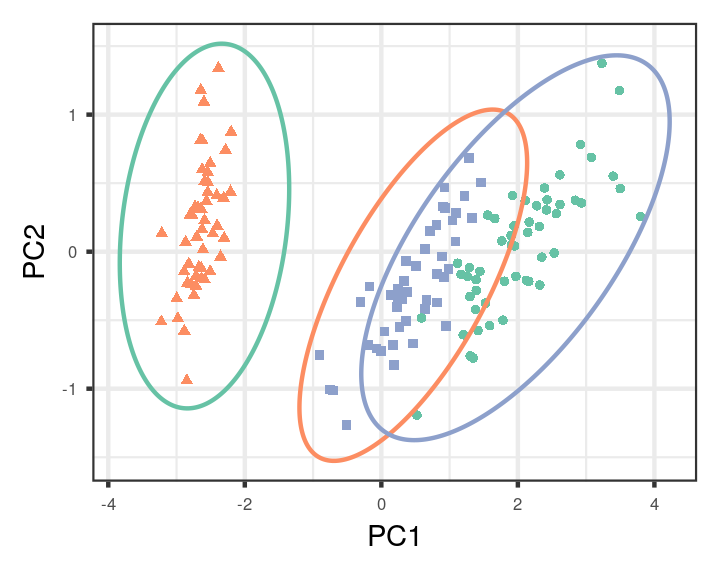
\includegraphics[width=0.588\linewidth,height=0.470\linewidth]{figure/iris_fit-1} 

}

\caption[The iris data in principal component space]{The iris data in principal component space. 
                      Colors denote inferred memberships and
                      ellipses are estimated covariances 
                      at $\alpha=6$.}\label{fig:iris_fit}
\end{figure}


\end{knitrout}


\begin{knitrout}
\definecolor{shadecolor}{rgb}{0.969, 0.969, 0.969}\color{fgcolor}\begin{figure}[!h]

{\centering 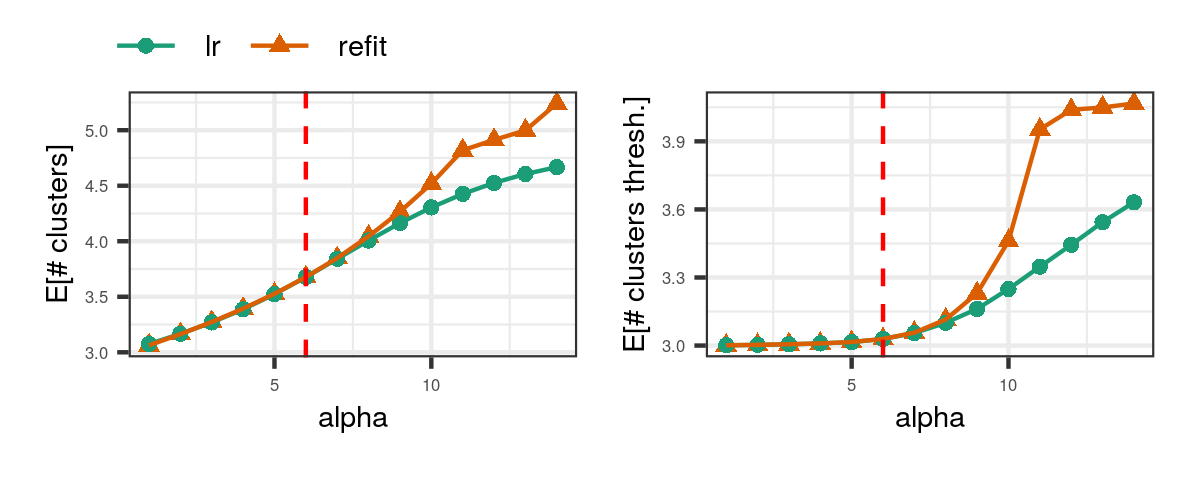
\includegraphics[width=0.980\linewidth,height=0.392\linewidth]{figure/iris_alpha_sens-1} 

}

\caption[The expected number of clusters in the iris data as $\alpha$ varies]{The expected number of clusters in the iris data as $\alpha$ varies. 
We compute the linear approximation at $\alpha=6$ and
extrapolate the expected number of clusters using the
linear approximation (green).
We compare against the expected number of clusters obtained by refitting the model at each $\alpha$ (orange). 
}\label{fig:iris_alpha_sens}
\end{figure}


\end{knitrout}



\begin{knitrout}
\definecolor{shadecolor}{rgb}{0.969, 0.969, 0.969}\color{fgcolor}\begin{figure}[!h]

{\centering 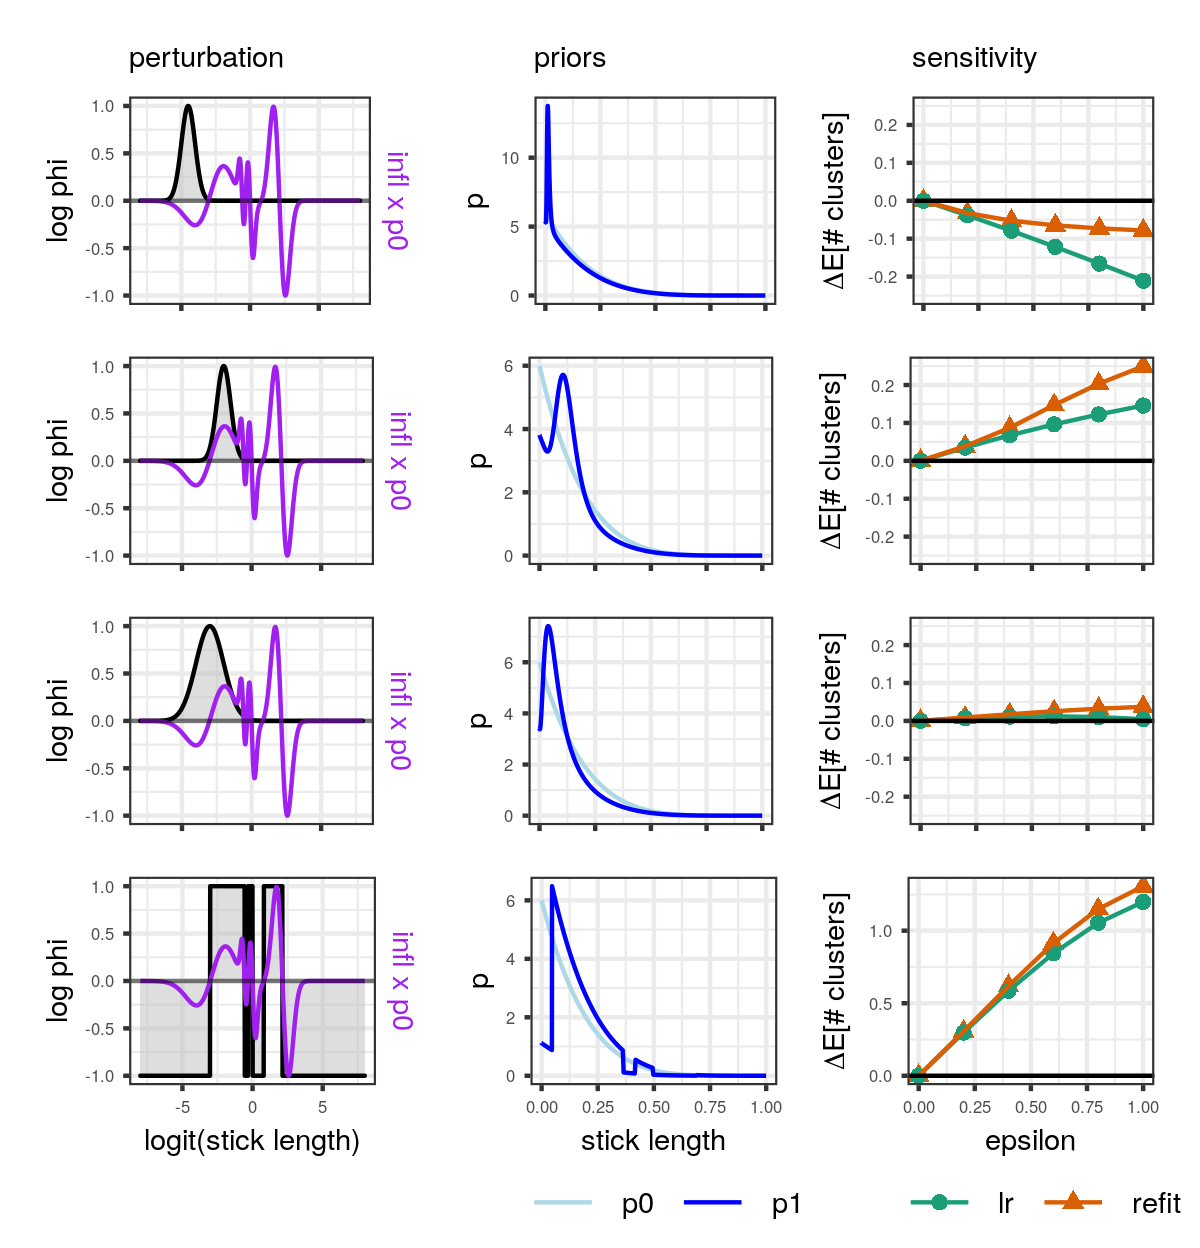
\includegraphics[width=0.980\linewidth,height=1.176\linewidth]{figure/iris_fsens-1} 

}

\caption[iris functional sensitivity ]{iris functional sensitivity }\label{fig:iris_fsens}
\end{figure}


\end{knitrout}


